\section{Bibliotecas Utilizadas}
\label{sec:bibs}

\subsection{Reconhecimento de Texto - Tesseract-OCR}

O reconhecimento de texto em imagens digitalizadas é parte
fundamental do projeto {\it webscan}, pois somente com o uso desta 
tecnica é possível se gerar documentos com páginas indexáveis.

Após pesquisar diversas bibliotecas (pesquisa apresentada no relatório I)
a biblioteca escolhida foi a 
Tesseract-OCR\footnote{http://code.google.com/p/tesseract-ocr}, que atualmente
possui código aberto e é mantida por um grande grupo.


\subsection{Exposição de métodos - Django}
O framework Python adotado para a exposição HTTP da lib {\it webscan} foi 
Django, pois além proporcionar recursos para um desenvolvimento ágil de 
aplicações Web ele ainda facilita a organização do código fonte de aplicações
deste tipo.
 
A separação de interesses sugerida nesse framework possui uma nomenclatura 
sutilmente diferente da nomenclatura comumente adotada por vários frameworks 
de aplicações Web. 

Ao invés do conhecido MVC (Model View and Controller) utiliza-se 
MTV (Model Template and View) assim o elemento `View' do MVC chama-se 
`Template' no MTV e o `Controller' do MVC chama-se `View' no MTV, dos 
quais o {\it webscan} utiliza apenas o elemento `View'. 

Consulte a documentação oficial\footnote{http://docs.djangoproject.com/en/dev/}
para informações detalhadas sobre Django.

\subsubsection{Processamento de requisições Web}

As requisições Web são mapeadas para uma 'View' através do arquivo urls.py.
Nesse arquivo podemos configurar expressões regulares que identificam cada 
uma das urls e associam a uma determinada função de callback (View). O 
código abaixo é um trecho do arquivo urls.py do módulo server do 
{\it webscan}: 

\begin{figure}[ht]
\begin{center}
\scalebox{0.65} {
    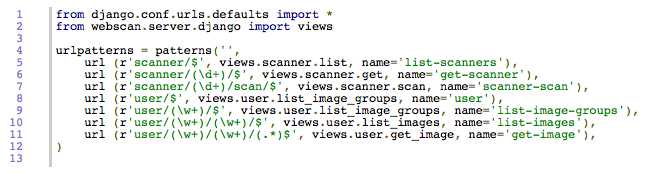
\includegraphics{imagens/urls.png}}
\end{center}
  \caption{Mapeamento de URL's - urls.py}
  \label{fig:urls}
\end{figure}

\subsection{Geração de PDF - Reportlab}

A biblioteca utilizada para geração de PDF foi a reportlab.
O código-fonte abaixo implementa a ação que gera um documento PDF apartir da 
imagem proviniente de um {\it pipeline} e seu respectivo texto OCR, se 
disponível.

\begin{figure}[ht]
\begin{center}
\scalebox{0.65} {
    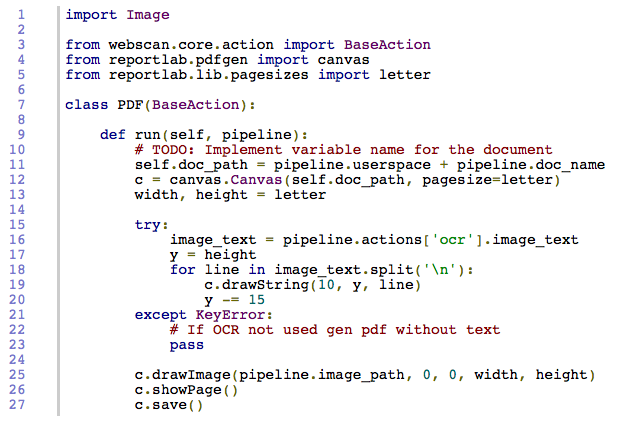
\includegraphics{imagens/pdf.png}}
\end{center}
  \caption{Action geradora de PDF's - pdf.py}
  \label{fig:urls}
\end{figure}


\subsection{Interface Web - JQuery}

O módulo UI, o qual é implementada a interface do projeto, utiliza-se apenas
de tecnologias web {\it client-side} tais como HTML, Javascript e CSS.

A utilização destas tecnologias, teoricamente, viabilizam a execução deste
artefato em qualquer plataforma que possua um navegador web compatível com elas,
porém esbarrando no problema de compatibilidade e adoção dos padrões 
internacionais W3C e ECMA.

Para que estes problemas fossem reduzidos a biblioteca 
JQuery\footnote{http://www.jquery.com} foi utilizada.
Em seu núcleo, a JQuery, implementa {\it wrappers} para os diferentes métodos
e detalhes implementados por cada navegador, ficando assim responsável por
garantir a compatibilidade do Javascript nos navegadores mais utilizados.
